\documentclass[
  english,          
  aspectratio=169,    % define the aspect ratio (169, 43)
  % handout=2on1,       % create handout with multiple slides (2on1, 4on1)
  % partpage=false,     % insert page at beginning of parts (true, false)
  % sectionpage=true,   % insert page at beginning of sections (true, false)
]{tumbeamer}

\usepackage{booktabs}
\usepackage{minted}
\usemintedstyle{colorful}
\usepackage{fontspec}
\setmonofont{JetBrainsMono}[
    Path=./jbmono/,
    Scale=0.85,
    Extension = .ttf,
    UprightFont=*-Regular,
    BoldFont=*-Bold,
    ItalicFont=*-Italic,
    BoldItalicFont=*-BoldItalic
    ]

\title{Docker resource management}
\subtitle{ACA Student Presentation }
\author{Roberto Castellotti}

\institute{\theDepartmentName\\\theUniversityName}
\date[14/12/2022]{December 14\textsuperscript{th}, 2022}

\footline{\insertauthor~|~\insertshorttitle~|~\insertshortdate}

\TUMbeamersetup{
  title page = TUM tower,         % style of the title page
  part page = TUM toc,            % style of part pages
  section page = TUM toc,         % style of section pages
  content page = TUM more space,  % style of normal content pages
  tower scale = 1.0,              % scaling factor of TUM tower (if used)
  headline = TUM threeliner,      % which variation of headline to use
  footline = TUM default,         % which variation of footline to use
  % configure on which pages headlines and footlines should be printed
  headline on = {title page},
  footline on = {every page, title page=false},
}
\begin{document}

\maketitle

\begin{frame}{Quick questions}
  \begin{itemize}
    \item Who has ever heard of Docker?
    \item Who used Docker at least once?
    \item Who uses Docker in their daily life?
    \item Who knows that  tools similar to Docker exist? (or focusing on subtasks)
    \item Who has seen this slide at least 5 times?
  \end{itemize}
\end{frame}

\begin{frame}{Containers vs VMs (once again)}
\begin{figure}
    \centering
    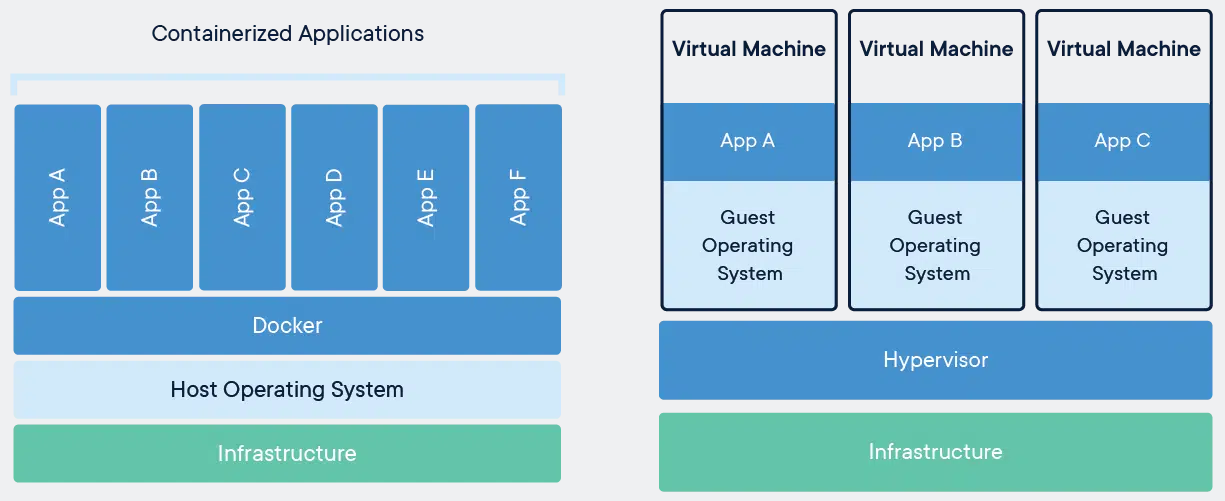
\includegraphics[width=0.8\textwidth]{container-vs-vms.png}
    \caption{from: https://www.docker.com/resources/what-container/ }
    \label{fig:my_label}
\end{figure}
    
\end{frame}

\begin{frame}{"Docker"}
The \href{https://opencontainers.org/}{Open Container Initiative} is an open governance structure for the express purpose of creating open industry standards around container formats and runtimes.
\centering \begin{tabular}{ccc}

\includegraphics[width=.1\linewidth]{docker.png} & 

\includegraphics[width=.2\linewidth]{podman.png} & 

\includegraphics[width=.2\linewidth]{buildah.png}\\

\includegraphics[width=.2\linewidth]{skopeo.png} &

\includegraphics[width=.2\linewidth]{packer.png} &

\includegraphics[width=.2\linewidth]{kaniko.png}\\

\includegraphics[width=.2\linewidth]{containerd.png} & 

\includegraphics[width=.1\linewidth]{finch.png} & 
\end{tabular}
\end{frame}

\begin{frame}{How do containers provide isolation?}
"Applications are safer in containers and Docker provides the strongest default isolation capabilities in the industry" \footnote{\href{https://www.docker.com/resources/what-container/}{https://www.docker.com/resources/what-container/}}
\vspace{15mm}
\begin{itemize}
    \item linux namespaces (limits what you see)
    \item cgroups (limits what you can use use)
\end{itemize}
\end{frame}

\begin{frame}{Linux Namespaces}
Namespaces are a feature of the Linux kernel that partitions kernel resources such that one set of processes sees one set of resources while another set of processes sees a different set of resources.... Examples of such resources are process IDs, hostnames, user IDs, file names, and some names associated with network access, and interprocess communication.\footnote{\href{https://en.wikipedia.org/wiki/Linux_namespaces}{https://en.wikipedia.org/wiki/Linux\_namespaces}}
\vspace{8mm}
\begin{itemize}
    \item inspired by the wider namespace functionality used heavily throughout Plan 9 from Bell Labs.
    \item 2002: initial work on namespaces introduced in Linux mainline kernel 2.4.19 
    \item February 2013: user namespaces are introduced in Linux mainline kernel 3.8 (we now have adequate container support functionality)
\end{itemize}
\end{frame}

\begin{frame}{Type of Linux Namespaces}
\begin{itemize}
    \item \textbf{User} namespaces isolate User and group IDs
    \item \textbf{PID} namespaces isolate process IDs (nested trees; PID 1 in a subtree)
    \item \textbf{Mount} namespaces isolate mount points
    \item \textbf{Network} namespaces isolate Network devices, stacks, ports
    \item some others, check \texttt{man} page
\end{itemize}
\end{frame}

\begin{frame}[fragile]{Let's get our hands dirty, user namespace(1/2)}
\begin{minted}[fontsize=\footnotesize]{bash}
# outside the namespace
rc@s369 ~/t/aca> whoami
rc
rc@s369 ~/t/aca> id
uid=1000(rc) gid=1000(rc) groups=1000(rc), ...
rc@s369 ~/t/aca> sudo unshare --user
# inside the namespace
nobody@s369:/home/rc/tum-exams/aca$ whoami
nobody
nobody@s369:/home/rc/tum-exams/aca$ id
uid=65534(nobody) gid=65534(nogroup) groups=65534(nogroup)
nobody@s369:/home/rc/tum-exams/aca$ 

\end{minted}

Who is \texttt{nobody}? 
\small "If a user ID has no mapping inside the namespace, then system calls that return user IDs return the value defined in the file \texttt{/proc/sys/kernel/overflowuid}, which on a standard system defaults to the value 65534."\footnote{\href{https://lwn.net/Articles/532593/}{https://lwn.net/Articles/532593/}}

\end{frame}

\begin{frame}[fragile]{Let's get our hands dirty, user namespace (2/2)}
\begin{minted}[fontsize=\footnotesize]{bash}
# outside the namespace
rc@s369 ~/t/aca> whoami
rc
rc@s369 ~> id
uid=1000(rc) gid=1000(rc) groups=1000(rc), ...
rc@s369 ~> sudo unshare --user --map-root-user
# inside the namespace
root@s369:/home/rc# whoami
root
root@s369:/home/rc# id
uid=0(root) gid=0(root) groups=0(root)
\end{minted}
This is probably what you need if you are creating a user namespace.
\end{frame}

\begin{frame}[fragile]{Let's get our hands dirty, mount namespace}
\begin{minted}[fontsize=\footnotesize]{bash}
rc@s369 ~> sudo unshare --mount
# inside the namespace
root@s369:/home/rc# mount -t tmpfs tmpfs /mnt
root@s369:/home/rc# echo "I love ACA student presentations!" > /mnt/aca.txt
root@s369:/home/rc# cat /mnt/aca.txt
I love ACA student presentations!
root@s369:/home/rc# 
logout
# outside of namespace
rc@s369 ~> ls -l /mnt/aca.txt
ls: cannot access '/mnt/aca.txt': No such file or directory
rc@s369 ~ [2]>
\end{minted}
\end{frame}

\begin{frame}[fragile]{Let's get our hands dirty, net namespace (1/2)}
\begin{minted}[fontsize=\footnotesize]{bash}
# outside the namespace
rc@s369 ~> ip a
1: lo: <LOOPBACK,UP,LOWER_UP> mtu 65536 qdisc noqueue state UNKNOWN group default qlen 1000
    link/loopback 00:00:00:00:00:00 brd 00:00:00:00:00:00
    inet 127.0.0.1/8 scope host lo
       valid_lft forever preferred_lft forever
    inet6 ::1/128 scope host 
       valid_lft forever preferred_lft forever
2: enp0s31f6: <NO-CARRIER,BROADCAST,MULTICAST,UP> mtu 1500 qdisc fq_codel state DOWN group default qlen 1000
    link/ether 54:e1:ad:5d:1c:6e brd ff:ff:ff:ff:ff:ff
.... i should probably clean this up :)
rc@s369 ~> ip route
default via 131.159.223.254 dev wlp4s0 proto dhcp metric 600 
131.159.192.0/19 dev wlp4s0 proto kernel scope link src 131.159.218.200 metric 600 
169.254.0.0/16 dev br-0d5fb61239aa scope link metric 1000 
172.17.0.0/16 dev docker0 proto kernel scope link src 172.17.0.1 linkdown 
172.18.0.0/16 dev br-0d5fb61239aa proto kernel scope link src 172.18.0.1 
\end{minted}
\end{frame}

\begin{frame}[fragile]{Let's get our hands dirty, net namespace (2/2)}
\begin{minted}[fontsize=\footnotesize]{bash}
rc@s369 ~> sudo unshare --net  /bin/bash
# inside the namespace
root@s369:/home/rc# ip a
1: lo: <LOOPBACK> mtu 65536 qdisc noop state DOWN group default qlen 1000
    link/loopback 00:00:00:00:00:00 brd 00:00:00:00:00:00
root@s369:/home/rc# iptables --list-rules
-P INPUT ACCEPT
-P FORWARD ACCEPT
-P OUTPUT ACCEPT
root@s369:/home/rc# ip route
root@s369:/home/rc# 
\end{minted}
\end{frame}

\begin{frame}[fragile]{Let's get our hands dirty, pid namespace (1/2)}
\begin{minted}[fontsize=\scriptsize]{bash}
rc@s369 ~> ps -aux | head -2
USER         PID %CPU %MEM    VSZ   RSS TTY      STAT START   TIME COMMAND
root           1  0.0  0.0 168412 13844 ?        Ss   09:56   0:04 /sbin/init splash
rc@s369 ~> ps -aux | wc -l
324
rc@s369 ~> sudo unshare --fork --pid   /bin/bash
root@s369:/home/rc# ps -aux | wc -l
328
root@s369:/home/rc# ps -aux | head -2
USER         PID %CPU %MEM    VSZ   RSS TTY      STAT START   TIME COMMAND
root           1  0.0  0.0 168412 13844 ?        Ss   09:56   0:04 /sbin/init splash
rc@s369 ~> sudo unshare --fork --pid --mount-proc  /bin/bash
root@s369:/home/rc# ps -aux
USER         PID %CPU %MEM    VSZ   RSS TTY      STAT START   TIME COMMAND
root           1  0.0  0.0  10236  4132 pts/4    S    18:53   0:00 /bin/bash
root           8  0.0  0.0  12940  3720 pts/4    R+   18:53   0:00 ps -aux
\end{minted}
Why this happens? 
\end{frame}

\begin{frame}[fragile]{Let's get our hands dirty, pid namespace (2/2)}
\footnotesize The \texttt{ps} program uses the procfs virtual file system to obtain information about the current processes in the system. This filesystem is mounted in the \texttt{/proc} directory. However, in the new namespace this mountpoint describes the processes from the root PID namespace.
\begin{minted}[fontsize=\scriptsize]{bash}
rc@s369:~$ echo $$
45460
rc@s369:~$ ls /proc/45460
arch_status         cwd        mem            patch_state   stat
attr                environ    mountinfo      personality   statm
autogroup           exe        mounts         projid_map    status
auxv                fd         mountstats     root          syscall
cgroup              fdinfo     net            sched         task
clear_refs          gid_map    ns             schedstat     timens_offsets
cmdline             io         numa_maps      sessionid     timers
comm                limits     oom_adj        setgroups     timerslack_ns
coredump_filter     loginuid   oom_score      smaps         uid_map
cpu_resctrl_groups  map_files  oom_score_adj  smaps_rollup  wchan
cpuset              maps       pagemap        stack
rc@s369:~$ ls /proc/45460/ns
cgroup  mnt  pid               time               user
ipc     net  pid_for_children  time_for_children  uts
\end{minted}
\end{frame}

\begin{frame}{Cgroups}

Cgroups is a Linux kernel feature that limits, accounts for, and isolates the resource usage (CPU, memory, disk I/O, network, etc.) of a collection of processes.\footnote{\href{https://en.wikipedia.org/wiki/Cgroups}{https://en.wikipedia.org/wiki/Cgroups}}
\vspace{10mm}
\begin{itemize}
    \item 2006: engineers at Google start working of this feature
    \item January 2008: cgroups functionality is merged in the Linux mainline kernel (2.6.24)
    \item December 2016: cgroups v2 is merged in Linux mainline kernel (4.5) with some improvements
\end{itemize}
\end{frame}

\begin{frame}{Cgroup controllers}
\begin{itemize}
% \begin{itemize}[<+->]
    \item \textbf{cpu}: grants a minimun number of "CPU shares" when system is busy
    \begin{itemize}
        \item \small from 3.2: CPU "bandwidth" control 
    \end{itemize}
    \item \textbf{devices}: supports controlling which processes may create (mknod) devices as well as open them for reading or writing.
    \item \textbf{cpuacct}: provides accounting for CPU usage by groups of processes.
    \item \textbf{pids}: permits limiting the number of process that may be created in a cgroup (and its descendants).
    \item \textbf{net\_cls}: places a classid on network packets created by a cgroup.  
    \item \textbf{memory}: supports reporting and limiting of process memory, kernel memory, and swap used by cgroups.
    \item \textbf{blkio}: controls and limits access to specified block devices.
    \item \textbf{hugetlb}, \textbf{rdma}, \textbf{cpuset}, \textbf{cpu\_prio}, \textbf{net\_prio}, \textbf{perf\_event}, \textbf{freezer}
    
\end{itemize}
\end{frame}


\begin{frame}[fragile]{Memory controller hands on}
\begin{minted}{bash}
root@s369:/# mkdir /sys/fs/cgroup/memory/cgtest
root@s369:/# echo 5000 > /sys/fs/cgroup/memory/cgtest/memory.limit_in_bytes
root@s369:/# cat /sys/fs/cgroup/memory/cgtest/memory.limit_in_bytes 
4096
\end{minted}
\vspace{3mm}
now let's create a simple script \textt{test.sh}
\vspace{3mm}

\begin{minted}{bash}
#!/bin/bash

while [ 1 ]; do
        echo "I love Advanced Computer Networking Student Presentations!"
        sleep 20
done
\end{minted}

\end{frame}
\begin{frame}[fragile]{Memory controller hands on}
\begin{minted}{bash}
rc@s369:~$ sh ~/test.sh &
[1] 9668
root@s369:/# echo 9668 > /sys/fs/cgroup/memory/cgtest/cgroup.procs
rc@s369 ~> ps  9668
    PID TTY      STAT   TIME COMMAND
   9668 pts/2    S      0:00 sh /home/rc/test.sh
rc@s369 ~> ps  -o cgroup 9668
CGROUP
13:memory:/cgtest,11:pids:/user.slice/user-1000.slice/user@1000.service...
\end{minted}
\vspace{3mm}
after some time... \textt{test.sh}
\vspace{3mm}

\begin{minted}{bash}
rc@s369 ~> ps  9668
    PID TTY      STAT   TIME COMMAND
\end{minted}

What happened?
\end{frame}

\begin{frame}[fragile]{Memory controller hands on}
\begin{minted}{bash}
rc@s369:~$ sh ~/test.sh &
[1] 9668
root@s369:/# echo 9668 > /sys/fs/cgroup/memory/cgtest/cgroup.procs
rc@s369 ~> ps  9668
    PID TTY      STAT   TIME COMMAND
   9668 pts/2    S      0:00 sh /home/rc/test.sh
rc@s369 ~> ps  -o cgroup 9668
CGROUP
13:memory:/cgtest,11:pids:/user.slice/user-1000.slice/user@1000.service...
\end{minted}
\vspace{3mm}
after some time... \textt{test.sh}
\vspace{3mm}

\begin{minted}{bash}
rc@s369 ~> ps  9668
    PID TTY      STAT   TIME COMMAND
\end{minted}

What happened? There is a new sheriff in town! \href{https://docs.kernel.org/admin-guide/cgroup-v1/memory.html}{oom-killer}!
\end{frame}
\begin{frame}[fragile]{}
\begin{figure}
    \centering
    
\includegraphics[width=0.35\textwidth]{lets-see-meme.png}
\end{figure}
\end{frame}

\begin{frame}{further readings/talks}
\begin{itemize}
    \item \href{https://github.com/containerd/containerd/blob/main/docs/getting-started.md}{https://github.com/containerd/containerd/blob/main/docs/getting-started.md}
    \item \href{https://lwn.net/Articles/531114/}{https://lwn.net/Articles/531114/} (the entire series)
    \item \href{https://blog.quarkslab.com/digging-into-linux-namespaces-part-1.html}{https://blog.quarkslab.com/digging-into-linux-namespaces-part-1.html}
    \item \texttt{man} \{namespaces,cgroups\}
    \item \href{https://drewdevault.com/2022/11/12/In-praise-of-Plan-9.html}{https://drewdevault.com/2022/11/12/In-praise-of-Plan-9.html}
    \item \href{https://www.youtube.com/watch?v=sK5i-N34im8}{@jpetazzo - Cgroups, namespaces, and beyond: what are containers made from?}
    \item \href{https://www.youtube.com/watch?v=0kJPa-1FuoI}{Containers unplugged: Linux namespaces - Michael Kerrisk}
    \item \href{https://docs.kernel.org/admin-guide/cgroup-v1/cgroups.html}{https://docs.kernel.org/admin-guide/cgroup-v1/cgroups.html}
\end{itemize}
\end{frame}

\end{document}
